\documentclass[review]{elsarticle}

\usepackage{lineno,hyperref}
\modulolinenumbers[5]
%\usepackage[margin=2cm]{geometry}
\usepackage[justification=centering]{caption}
\usepackage{subfig}
\usepackage{multirow}
\usepackage{xcolor}
\usepackage{setspace}
\doublespacing
\renewcommand{\arraystretch}{1.1}
\journal{Pattern Recognition}

%%%%%%%%%%%%%%%%%%%%%%%
%% Elsevier bibliography styles
%%%%%%%%%%%%%%%%%%%%%%%
%% To change the style, put a % in front of the second line of the current style and
%% remove the % from the second line of the style you would like to use.
%%%%%%%%%%%%%%%%%%%%%%%

%% Numbered
%\bibliographystyle{model1-num-names}

%% Numbered without titles
%\bibliographystyle{model1a-num-names}

%% Harvard
%\bibliographystyle{model2-names.bst}\biboptions{authoryear}

%% Vancouver numbered
%\usepackage{numcompress}\bibliographystyle{model3-num-names}

%% Vancouver name/year
%\usepackage{numcompress}\bibliographystyle{model4-names}\biboptions{authoryear}

%% APA style
%\bibliographystyle{model5-names}\biboptions{authoryear}

%% AMA style
%\usepackage{numcompress}\bibliographystyle{model6-num-names}

%% `Elsevier LaTeX' style
\bibliographystyle{elsarticle-num}
%%%%%%%%%%%%%%%%%%%%%%%

\begin{document}

\begin{frontmatter}

%\title{Deep Learning for landmarking on morphometry anatomical images}
\title{Elementary Blocks Network to landmark anatomical images}
%\tnotetext[mytitlenote]{Fully documented templates are available in the elsarticle package on \href{http://www.ctan.org/tex-archive/macros/latex/contrib/elsarticle}{CTAN}.}

%% Group authors per affiliation:
%\author{Elsevier\fnref{myfootnote}}
%\address{Radarweg 29, Amsterdam}
%\fntext[myfootnote]{Since 1880.}

%% or include affiliations in footnotes:
\author[labri,itdlu]{Le Van Linh\corref{cor1}}
\ead{van-linh.le@labri.fr}
\author[labri]{Beurton-Aimar Marie\fnref{ba}}
\ead{beurton@labri.fr}
\author[labri]{Zemmari Akka}
\ead{zemmari@labri.fr}
\author[igepp]{Parisey Nicolas\fnref{ba}}
\ead{nicolas.parisey@inra.fr}

\fntext[ba]{both authors contributed equally to this work.}
\cortext[cor1]{Corresponding author} 

\address[labri]{University of Bordeaux, 351, cours de la Liberation, 33405 Talence, France}

%% %% or include affiliations in footnotes:
\address[igepp]{UMR 1349 IGEPP, BP 35327, 35653 Le Rheu, France}
%% \ead[url]{www.elsevier.com}
\address[itdlu]{Dalat University, Dalat, Lam Dong, Vietnam}

\begin{abstract}
In the previous century, deep learning has been introduced for the artificial intelligence program, but it is difficult to apply it in real cases because of the limitation of the resource at that time. In recent years, it has risen strongly because of improvements in computation performance. It
has been applied to solve problems in different domains such as
computer vision, speech recognition, or languages translation. Among
different types of deep learning architectures, Convolutional Neural
Networks have been most often used in computer vision for image
classification, object recognition, or key points detection and they
have brought amazing achievements. In this work, we propose a new
Convolutional Neural Network model based on composition of elementary
blocks, each elementary block is a sequence of layers,  to predict key points (landmarks) on 2D anatomical
biological images. Our proposed model has been trained and evaluated
on a dataset including the images of $3$ parts of $293$
beetles. During the experiments, the network has been tested in two
ways: training from scratch and applying fine-tuning process. In the fine-tuning step, to lead
the pre-training step, a large public dataset of key points on human
faces has been used. The obtained parameters have been then inserted
to re-train the model on beetle's images. The quality of predicted
landmarks is evaluated by comparing the coordinates distance between
predicted landmarks and manual ones which have been set by
biologists. The final results have been delivered to biologists and
they have confirmed that the quality of predicted landmarks is
statistically good enough to replace the manual landmarks for most of
the different morphometry analyses.

\end{abstract}

\begin{keyword}
Deep learning \sep CNN \sep fine-tuning \sep landmarks \sep key points detection \sep morphometry analysis
\end{keyword}

\end{frontmatter}

\linenumbers

\section{Introduction}
\label{sIntroduction}
In recent years, deep learning, which is a part of machine learning, is known as a
solution for difficult tasks in different domains \cite{lecun2015deep}. Computational model of deep
learning is composed of multiple layers to learn data
representation. Each layer may
contain different number of nodes, called \textit{neurons} which have
been inspired from the biological neural system
\cite{arbib2012brains}, and this is the main unit responsible for calculating at each layer. According, the neurons at a layer extract the representation of input data
which comes from the previous layers, then it computes a new
output to the next layer. Currently, deep learning has many kinds of
variant architectures and each of them has found success such as: Deep
Neural Network (DNN) to solve classification or data analysis
problems \cite{hinton2012deep, mikolov2011strategies}; Convolutional
Neural Network (CNN) in computer vision \cite{lecun1998gradient,
  krizhevsky2012imagenet,szegedy2015going}; Recurrent Neural Network
(RNN) on time sequences analysis \cite{lecun2015deep,jean2014using,
  sutskever2014sequence,collobert2011natural}. All of
them have exhibited impressive performance comparing to more classical
methods, for example, CNN is a specific
one for pre-processing data which have grid topology, such as time series (1-D), 2D and 3D images, or video. From the
first architecture \cite{lecun1998gradient} until now, many CNN models
have been proposed and have succeeded in different tasks of computer
vision such as image classification \cite{lecun1998gradient,
  krizhevsky2012imagenet,szegedy2015going}, object recognition
\cite{szegedy2015going,farabet2013learning,li2015convolutional}, and
key points detection \cite{liu2016fashion, sun2013deep,
  zhang2014facial, cintas2016automatic}.

In computer vision, key points detection is an important field. In
this field, algorithms try to find the key points, called Points of
Interest (PoI)  or landmarks through images. The landmarks are
considered as the points in the image that are invariant when the
scene changes, e.g. by some perspective projections. In biology, the
landmarks are most often manually annotated on digital images by
biologists. Depending on the objective of work and the studied object,
the number of landmarks may be different and their positions
 can be defined along the outline of the object or inside the
object. From landmarks coordinates, it is possible to extract object
features and to apply measure, for example, to detect human face
\cite{sun2013deep}, human pose \cite{huang2017coarse} or to measure out the organism anatomy.

In this work, we propose  a new composition of layers for a CNN
architecture, Elementary Blocks Network (EB-Net), to predict the
landmarks on biological species images. This model has been 
trained on the images of $3$ parts of $293$ beetles: pronotum, head, and elytra. We have also designed a
specific procedure to augment our dataset because several hundred
images are usually considered as a modest number to apply deep
learning methods. Finally in order to boost the prediction, we have
applied transfer-learning procedure with the help of a public human
facial key points database and fine-tuned our parameters model. The biologists have
asserted that the predicted landmarks were
statistically speaking good enough, in most of the cases, to replace the manual
landmarks. 

This paper is organized as followed: Section \ref{related_works}
presents the related works about deep learning and setting of
landmarks on 2D images. Section \ref{Sdataaug} describes the method to
augment our dataset. Section \ref{Sneuralnetwork} explains the design
of new network model. The first experiments of the network on each
dataset are presented in Section \ref{sexperiments}, and the last
section delivers all the final results including improvements provided
by the fine-tuning procedure.


\section{Related works}
\label{related_works}

In the middle of the previous century, deep learning algorithms
have been introduced as multiple layers of non-linear features by using statistical methods to select the best features to forward to the next layer. Additional, the backpropagation \cite{lecun1989backpropagation}, which has been introduced in the early $1960s$ in a inefficient and incomplete form, did not use to train the network at that time, instead, they used layer by layer least squares fitting. Until $1989$, LeCun \cite{lecun1998gradient} used convolutional networks in combination with backpropagation to classify handwritten digits (MNIST), and it was known as a first practical system for artificial
intelligence applications. However, several problems  appeared in
order to take into account real-world cases because of the limitation
of the memory size or computing power. Nowadays, huge improvements of
computing capacities, both in memory size and in computing time with
GPU programming, have opened a new perspective for deep learning. In
recent years, deep learning architectures have achieved remarkable
accomplishments in many domains such as computer vision
\cite{lecun1998gradient, krizhevsky2012imagenet,
  szegedy2015going,farabet2013learning,li2015convolutional, vu2018heritage}, speech
recognition \cite{hinton2012deep, mikolov2011strategies}, language
translation \cite{jean2014using, sutskever2014sequence}, natural
language processing \cite{lecun2015deep, collobert2011natural,
  collobert2008unified}. Especially in computer vision, deep learning,
specifically with CNN, has been used to achieve difficult tasks in
image analysis such as image classification, objects or key points
detection.


\subsection{Overview of Convolutional Neural Network}
A CNN is a feedforward network which takes the information following from the inputs to the outputs. Currently, CNNs have many variations, but it generally consists of several types of layers such as convolutional, pooling or fully connected layer. Fig. \ref{imgcnn_network} shows an overview of CNN network which inputs directly an image to several stages of convolutional and pooling layers. Then, the representation is feed into three fully connected layers. A dropout layer is inserted after the second fully connected layer to drop some nodes during the training process (blue nodes). Finally, the last fully connected layer gives output as the category label for the initial input image. This architecture could be seen as the most popular one. Reader interested in order details could read the review of Gu et al. \cite{gu2018recent}. 

\begin{figure}[!h]
	\centering
	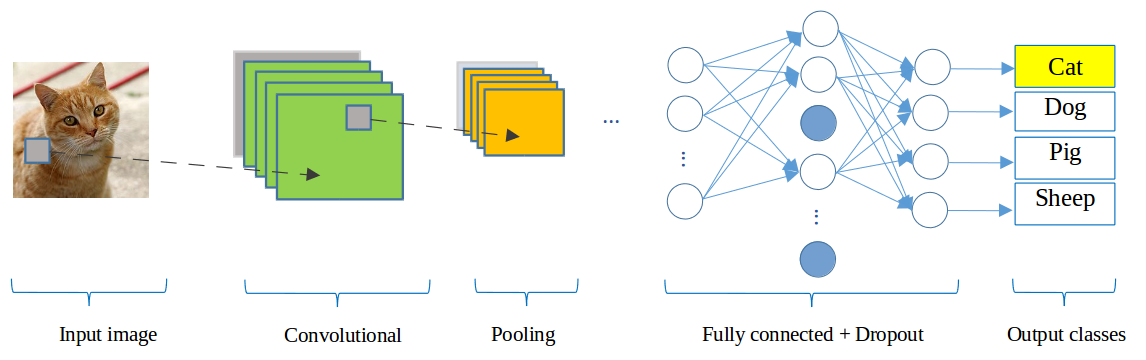
\includegraphics[scale=.3]{images/cnn_network_2}
	\caption{A CNN network for classification problem}
	\label{imgcnn_network}
\end{figure}

\subsection{State of the art in deep learning and key points detection}
LeNet \cite{lecun1998gradient} model is considered as the first
architecture of CNN. LeCun et al. \cite{lecun1998gradient} have used
it to classify the handwritten digits in cheques. LeNet exhibits a
standard architecture of a CNN which consists of $2$ convolutional
layers, pooling layers, followed by two fully connected layers. But to
be applied to realistic problems, this model requires huge computation
capacities and large amount of training data which were hardly
available in the early 2000s. In the last ten years, the computing
capabilities have drastically improved while, in the same time, a huge
amount of data became available, new models of neural networks
appeared well adapted to this new environment. One of the first ones
is AlexNet \cite{krizhevsky2012imagenet}, which is similar to LeNet
\cite{lecun1998gradient} but with a deeper structure: LeNet has 2
convolutional layers and 1 fully connected layer while AlexNet has 5
and 3, respectively. Furthermore, in AlexNet the activation functions
have been changed and dropout layers have been added to prevent the
over-fitting. AlexNet won the famous ImageNet Challenge\footnote{This
  is a challenge where evaluates algorithms for object detection and
  image classification.} in 2012. From the success of AlexNet, a lot
of different models have been proposed to improve the performance of
CNN, one can cite ZFNet  \cite{zeiler2014visualizing}, GoogLeNet
\cite{szegedy2015going}, VGGNet \cite{simonyan2014very}, or ResNet-50
\cite{he2016deep}. The main difference between these networks is that
their architectures became deeper and deeper by adding more layers,
e.g. ResNet-50, which won the champion of ILSVRC 2015, is deeper than
AlexNet around $20$ times.

 
Besides classification or recognition of objects, CNNs have been also
used to detect key points in 2D images. Liu et
al. \cite{liu2016fashion} have presented a method to predict the
positions of functional key points on fashion items such as the
corners of neckline, hemline and cuff. Yi Sun et
al. \cite{sun2013deep} have proposed a CNNs cascade to predict the
facial points belonging to the human face. Their model contains several CNNs which are linked together in a list
as a cascade. Three levels of the cascade are set to recognize the
human face from the global to local view with the objective to
increase the accuracy of predicted key points. In the same topic,
Zhanpeng Zhang et al. \cite{zhang2014facial} have proposed a
\textit{Tasks-Constrained Deep Convolutional Network} to join facial
landmarks detection problem with a set of related tasks, e.g. head
pose estimation, gender classification, age prediction, or facial
attribute inference. In their method, the input features have been
extracted by $4$ convolutional layers, $3$ pooling layers and $1$
fully connected layer which is shared by  multiple tasks in the
estimation step. Shaoli Huang et al. \cite{huang2017coarse} have
introduced a coarse-fine network to locate key points and to estimate
human poses. Their framework consists of the base convolutional layers
shared by two streams of key point detectors: the first stream, named
coarse stream, includes $3$ detector branches (3 stacks of Inception
modules \cite{szegedy2015going}) which are used to focus on capturing
local features and modeling spatial dependencies between human
parts. The second one, named fine stream, receives the  features which
are concatenated from the coarse stream and provides accurate
localization. Cintas et al. \cite{cintas2016automatic} have introduced
an architecture which enabled to recognize $45$ landmarks on human
ears. Their model includes $3$ times repeated of a structure consists of $2$ convolutional layers,
$1$ pooling layer, and $1$ dropout layer, to extract the
features. These structures are followed by $3$
fully connected layers. In the same context of key point detection, we
have developed a CNN to automatize landmarks prediction on beetle's
anatomies but before describing it, we will present the augmentation
procedure that we have defined for our dataset.



%As our work consists of a new architecture proposition for CNN, we have chosen to give in the next section some details about the definition of the different types of layers in CNN. The reader familiar to CNN can jump directly to the section about data augmentation.

\section{Data augmentation}
\label{Sdataaug}
From AlexNet to ResNet-50, the obtained success stories
\cite{krizhevsky2012imagenet,he2016deep} have proved that CNN models
produce better results on a large dataset but to use this technique,
the size of dataset remains a bottleneck and our own some hundred of
images are considered as modest for these models. So, it is important
to be able to provide a large dataset in order to learn more cases and to improve the learning ability of the network. Unfortunately, in some
application domains as this work in biology, providing a large dataset
is too costly. For this reason, one way to solve this problem is to
create misshapen data from real data and to add them to the training
set. Most often in image processing, dataset augmentation uses
operations like translation, rotation or scaling which are well known
to be efficient to generate new version of existing images. However,
this kind of operations are not useful in our case because the
analysis of images by CNN (convoluted) are usually invariant to
translation or rotation. So, we prefered to rely on method changing
color space values to obtain misshapen images.

Our image set is in RGB color map, the first procedure consists of
changing the value of one color channel of the three channels in the
original image to generate a new image. A constant value is sampled in
an uniform distribution $\in [1, 255]$ to obtain a new value caped at
$255$. For example, Fig. \ref{figaug1} shows the three images which
are generated  when a constant $c = 10$ is added to each channel of an
original image. Following this way, we can generate three new versions
of only one image.

\begin{figure}[h]
	\centering
	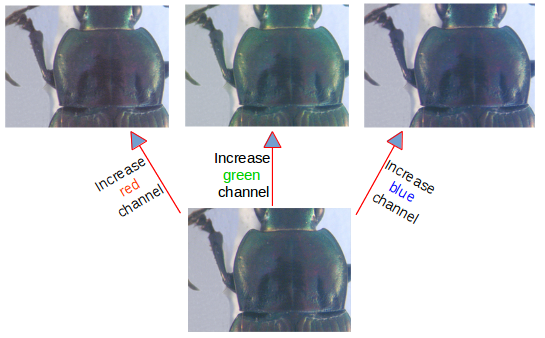
\includegraphics[scale=0.4]{images/inc_channels}
	\caption{A constant $c = 10$ has been added to each channel of an original image}
	\label{figaug1}
\end{figure}

In the second procedure, each channel is considered separately and one
grayscale image is generated for it (Fig. \ref{figaug2}). Consequently, we
obtain 3 new images (single channel) from an original one. At the end
of the process, $6$ versions of an original image are made. In total,
the new data set contains $293 \times 7 = 2051$ images for each
anatomical part of beetle (an original image and six misshapen ones).

\begin{figure}[h]
	\centering
	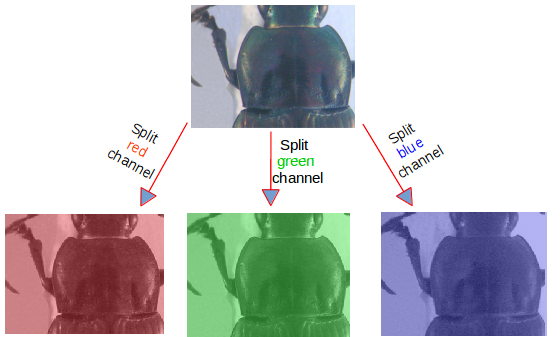
\includegraphics[scale=0.4]{images/sp_channels}
	\caption{Three channels (red, green, blue) are separated from original image}
	\label{figaug2}
\end{figure}
%However, we have not used all images for training and validation. So, we have chosen $260$ original images and their generations ($1820$ images) of each dataset for training and validation processes, the remaining images ($33$ original images) are used for test process. In practical, to obtain a fast convergence during the computing, it is useful to normalize the brightness of the images to $[0,1]$ instead of $[0, 255]$ and the coordinates of the landmarks have been also normalized \cite{lecun2012efficient}.

\section{Network architectures designing}
\label{Sneuralnetwork}
As we have presented previously, several CNN architectures are
available from literature and tool libraries. It is always possible
to adapt them to a specific application by changing the parameters
values or by modifying the arrangement of layers. Indeed, several
trials have been achieved before to obtain a satisfying model
dedicated to landmarks estimation. In this section, we present three
versions of the model that we have designed to solve this task. As
usual, we have combined the classical layer types to build the model,
e.g. convolutional, maximum pooling, dropout, and fully-connected
layers.


The first architecture has been a very classical one
(Fig. \ref{fignet1}). It receives an input image with the size of $1
\times 192 \times 256$, then it is composed by $3$ repeated structures
of a convolutional (CONV) layer followed by a maximum pooling (POOL)
layer. In most of CNNs, the parameters of CONV layers have been set to
increase the depth of the feature maps from the first  to the last
layer. This is done by setting the number of filters at each CONV
layer. In this first model, the depths of the CONV layers increase
from $32, 64, $ to $128$ and with different size of the kernels: $3
\times 3$, $2 \times 2$ and $2 \times 2$, respectively. Inserting POOL
layers after a CONV layers is usually done. The POOL layers
progressively reduce the spatial size of the representation, reduce
the number of parameters, computation in the network, and also prevent over-fitting. The operations of POOL layers are independent
for each depth slice of their inputs. In our model, we have used the
most common form for one POOL layer: a filter with size of $2 \times
2$ and a stride equal to the size of filter have been applied. At the
end of the model, $3$ fully-connected (FC) layers have been added to extract the global
relationship between the features and to proceed the outputs. The
first two FC layers have been applied the activation functions to make
sure these nodes interact well and to take into account all possible
dependencies at the feature level. The outputs of the FC layers are
$500, 500$ and $16$. The output of the last FC layer corresponds to
the coordinates ($x$ and $y$) of $8$ landmarks which we would like to
predict on pronotum part. Nevertheless, the obtained results with this
architecture has not been considered good enough to continue to use
it. One of the main problems is the presence of over-fitting during
the training process (Detailed results will be discussed in Section
\ref{sexperiments}).

\begin{figure}[!h]
	\centering
	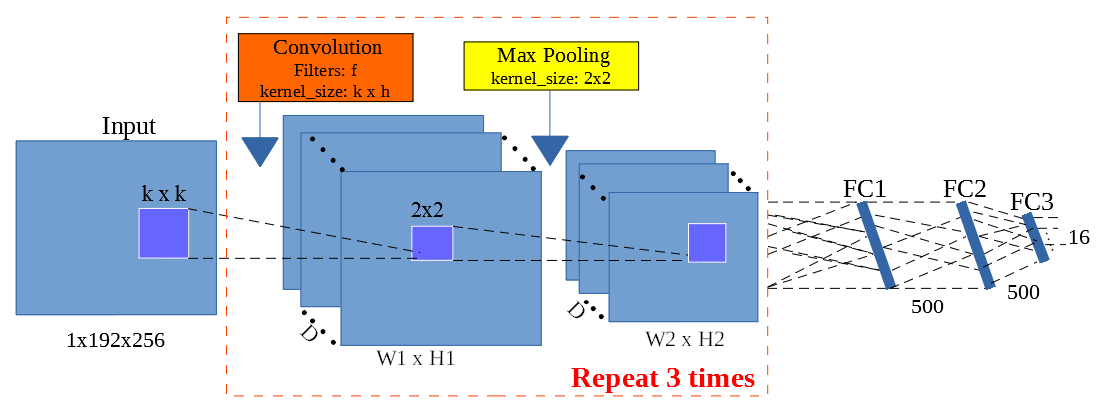
\includegraphics[width=0.98\textwidth]{images/model1}
	\caption{The architecture of the first model}
	\label{fignet1}
\end{figure}

The second model has kept the same architecture of the first model but
the number of output of the two FC layers has been increased to
$1000$. Increasing the value at FC layers could allow to get more
features from CONV layer without requirements of computing
resources. However, the obtained results remained not satisfying, it
will be discussed also in the result section (Section
\ref{sexperiments}).


To build the third architecture, we have defined the
\textit{Elementary Block} (EB). An EB is defined as a sequence of $1$
CONV ($C_{i}$), $1$ maximum POOL ($P_i$) and $1$ dropout ($D_i$)
layers (Fig. \ref{figelementary}). The dropout layer has been added to
prevent over-fitting by adding a step to remove some nodes. This has
significantly reduced overfitting and over performed the other
regularization methods \cite{srivastava2014dropout}.


\begin{figure}[h]
	\centering
	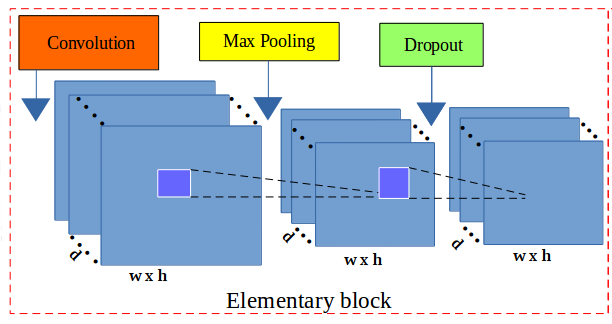
\includegraphics[width=0.5\textwidth]{images/elementary_block}
	\caption{The layers in an elementary block. It includes a CONV layer (orange), a maximum POOL layer (yellow) and a DROP layer (green).}
	\label{figelementary}
\end{figure}

Fig. \ref{fignet3} illustrates the structure of the third
architecture. For our purpose, we have assembled \textbf{3 elementary
  blocks} which are the main components of \textbf{EB-Net}. The
parameters for each layer in each elementary block are described as
below, the list of values follows the order of elementary blocks ($i =
[1..3]$):

\begin{itemize}
	\item CONV layers:
	\begin{itemize}
		\item Number of filters: $32, 64, $ and $128$
		\item Kernel filter sizes: $(3 \times 3), (2 \times 2), $ and $(2 \times 2)$
		\item Stride values: $1, 1, $ and $1$ 
	\end{itemize}
	\item POOL layers:
		\begin{itemize}
			\item Kernel filter sizes: $(2 \times 2), (2 \times 2), $ and $(2 \times 2)$
			\item Stride values: $2, 2, $ and $2$
		\end{itemize}
	\item DROP layers:
		\begin{itemize}
			\item Probabilites: $0.1, 0.2, $ and $0.3$
		\end{itemize}
\end{itemize}

For the FC layers, FC1 and FC2 have $1000$ outputs, the last FC layer (FC3) has $16$ outputs. As usual, a dropout layer is inserted between FC1 and FC2 with a probability equal to $0.5$.

\begin{figure}[h]
	\centering
	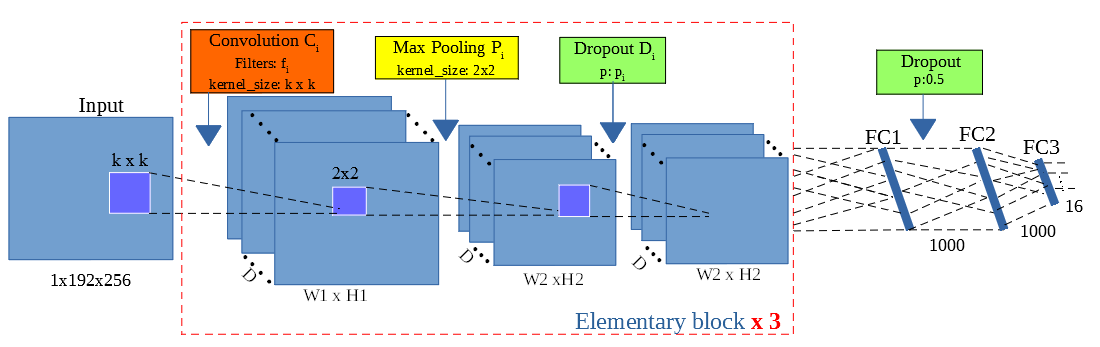
\includegraphics[width=0.99\textwidth]{images/model3}
	\caption{The architecture of EB-Net}
	\label{fignet3}
\end{figure}

The core of CNN is training over iterations. In each iteration, the features of images are computed in two phases: forward and backward. In the forward phase, the features are computed following the order of the layer in the network. In the backward phase, the values of learnable parameters are computed and updated to increase the accuracy of the network by using an optimizer. There are many ways to
optimize the learning algorithm, but gradient descent
\cite{lecun2012efficient} is currently a good choice to reduce the
loss in neural network. The core idea is to follow the gradient until
reaching a minimum of the cost function. So, we have chosen gradient
descent in the backward phase to update the values of learnable
parameters. EB-Net was designed to use a learning rate initialize at
$0.03$ and to stop at $0.00001$, while the momentum rateS was updated from
$0.9$ to $0.9999$. The values were updated over training time to fit
with the number of epochs \footnote{An epoch is a single pass through
  the full training set} by applying parameters adjustment during the
training. The architecture implementation has been written in Lasagne
framework \cite{lasagne} in Python code. More information about the
model can be obtained from the repository on GitHub:
\texttt{https://github.com/linhlevandlu/CNN\_Beetles\_Landmarks}

\section{Experiments and results}
\label{sexperiments}
Fig. \ref{fig5parts} presents the $5$ different beetle parts belonging
to our dataset. The two first ones (from the left side) have been
studied in previous work based on image processing techniques
to work with segmentable images \cite{le2017maelab}. The choice to
turn to deep learning methods for the three remained ones have
been motivated by the high difficulty to segment them, as we can
observed in Fig. \ref{fig5parts}. Segmentation is most often a
requirement to apply traditonal image processing methods and can be a
bootleneck to achieve treatments. Using convolutional networks does not
require this operation and provide solution to overcome this
problem. Pronotum was the first part we analyzed with deep learning and the presented results mainly concern
these images.

\begin{figure}[h]
	\centering
	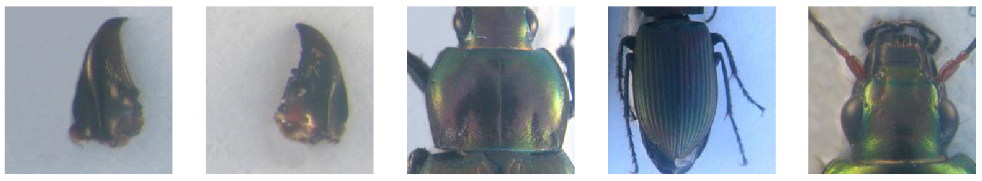
\includegraphics[width=0.97\textwidth]{images/images5parts}
	\caption{The image in each part of beetle. From left to right:
          left, right mandibles, pronotum, elytra and head.}
	\label{fig5parts}
\end{figure}
The networks have been trained in $5, 000$ epochs on Linux OS by using
NVIDIA TITAN X cards. During the training, the images are chosen
randomly from the dataset with a ratio of $60\%$ for training and
$40\%$ for validation. For each pronotum image, a set of $8$ manual
landmarks is available. They have been set by biologists and are
considered as the ground truth for the evaluation. In deep learning,
many kinds of loss functions can be considered depending on the
class of problem solving by the network, we have considered Root Mean
Square Error (RMSE) because it is usually used for regression problems
where the outputs are not discrete values as in the case of landmarks coordinates.

In order to predict landmarks for all pronotum images, we have applied
\textit{cross-validation} procedure to choose the test images, we call
it \textit{round}. For each round, we have decided to choose $33$
images for testing step and the $260$ remaining images have been used to train and to validate the model. So, $9$ rounds will be necessary to predict
all landmarks. Of course, this dataset has been
augmented as described in Section \ref{Sdataaug} to provide $1820$ images for these $2$
steps.

\begin{figure}[h!]
    \centering
    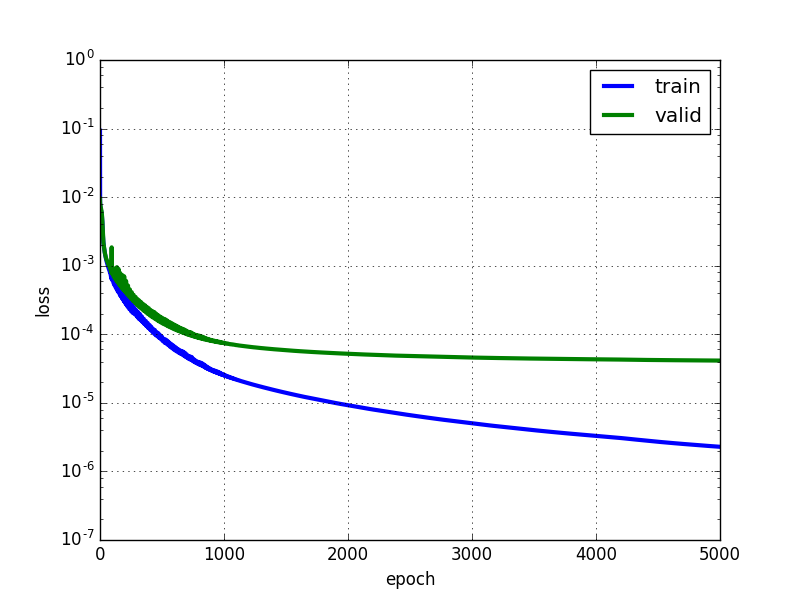
\includegraphics[width=0.6\textwidth]{images/model1_loss}
    \caption{The losses (training and validation) of the $1^{st}$ model. The
      blue curve presents the RMSE errors of training process while
      green curve is the validation errors.}
    \label{figlosses}
\end{figure}

As it has been mentioned in Section \ref{Sneuralnetwork}, the first
and the second model exhibit over-fitting
behavior. Fig. \ref{figlosses} shows the different curves of the
losses during training and validation step in the first architecture model. The blue curve presents
the RMSE error of training process while green curve is the
validation error. Clearly, over-fitting has appeared in the first
model, e.g. training loss is able to decrease but validation
loss is stable. In the second one, no concrete change appears in the curves even the parameters of fully-connected layers were modified.

\begin{figure}[h!]
    \centering
    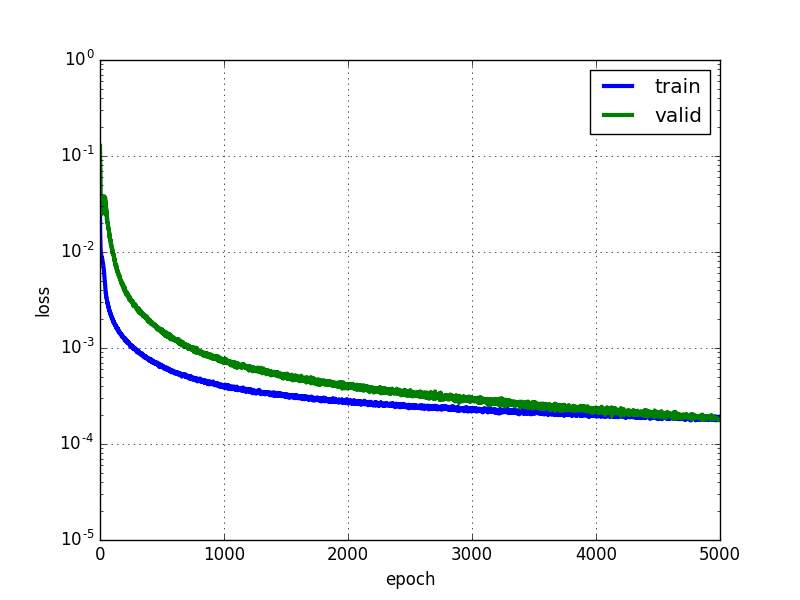
\includegraphics[width=0.6\textwidth]{images/model3_loss}
    \caption{The losses (training and validation) of EB-Net}
    \label{figloss3}
\end{figure}

Fig. \ref{figloss3} illustrates the losses during the training of the
third model, EB-Net. One can note that after several epochs, the
two-loss values become close and the over-fitting disappears, we can
assume that the addition of Dropout sequence inside elementary block works well to prevent over-fitting and improves the accuracy of the model greatly.

Table \ref{tbltrainingloss} resumes the losses of $9$ rounds when we
trained EB-Net on pronotum images. Clearly, the training/validation
losses among rounds are tiny and stable.

\begin{table}[h!]
	\centering
	\begin{tabular}{l l l}
	Round & Training loss & Validation loss \\ \hline
	1 & 0.00018 & 0.00019  \\ \hline
	2 & 0.00019 & 0.00021 \\ \hline
	3 & 0.00019 & 0.00026 \\ \hline
	4 & 0.00021 & 0.00029 \\ \hline
	5 & 0.00021 & 0.00029 \\ \hline
	6 & 0.00019 & 0.00018 \\ \hline
	7 & 0.00018 & 0.00018 \\ \hline
	8 & 0.00018 & 0.00021 \\ \hline
	9 & 0.00020 & 0.00027 \\ \hline
	\end{tabular}
	\caption{\small{The losses during training the third model on pronotum images}}
	\label{tbltrainingloss}
\end{table}
%To evaluate the coordinates of predicted landmarks, the correlation
%metrics between the manual landmarks and corresponding predicted ones
%have been computed. Table. \ref{tblcorrelation} shows the correlation
%scores of $3$ metrics (using \textit{scikit-learn}
%\cite{pedregosa2011scikit}), e.g. coefficient of determination
%($r^2$), explained variance (EV), and Pearson correlation. These
%three metrics are both appropriate for our dataset type. The results
%closed to $1$ show that the predicted coordinates are very close with
%the ground truth. It proves that our prediction is good enough to
%replace manual landmarks in statistical analysis of pronotum
%morphology. However, standing on the side of image processing, seeing
%the real coordinates on images is more appropriate than statistical
%results. So, the distances (in pixels) between manual coordinates and
%predicted coordinates have been calculated for all images. Then, the
%average distance for each landmark has been computed.

To evaluate the coordinates of predicted landmarks, the Pearson
correlation  metric  between predicted and manual landmarks has been
calculated for each dimension (x and y). Table \ref {tblcorrelation}
shows the obtained results. The average value of the coordinates
correlation (both x and y) is in the first row, variance,
minimum and maximum of correlation scores are given in the next
rows. One can note that the correlation is strongly positive in each
case with a very small variance, proving that each individual
coordinate is well predicted.
\begin{table}[htbp]
	\centering
	\begin{tabular}{ | l | c | c | }
\hline
	& X-dimension & Y-dimension  \  \\ \hline
	Mean & 0.8116 & 0.9438 \\ \hline
	Variance  & 0.0020 & 0.0006 \\ \hline
	Min  & 0.7474 & 0.9063 \\ \hline
	Max  & 0.8577 & 0.9638 \\ \hline
\end{tabular}
	\caption{Statistical indicators on Pearson correlation between manual and predicted landmarks}
	\label{tblcorrelation}
\end{table}

Standing on the side of the users, biologists would like to
obtain an acceptable position of the landmark when they look at the
images. So, the distances (in pixels) between manual coordinates and predicted
ones have been calculated for all images. Then, the average
distance for each landmark has been
computed. Table \ref{tblavgpronotum} shows the average distances by
landmarks on all images of pronotum dataset. With the images
resolution $256 \times 192$, we can consider that an error around $1\%$
(corresponding to $2$ pixels) could 
be an acceptable error. Unhappily, our results exhibit average
distance of $4$ pixels in the best case, landmark $1$ and more than
$5$ pixels in the worse case, landmark $6$.
\begin{table}[htbp]
	\centering	
	\begin{tabular}{|c|c|}
		\hline
		\textbf{Landmark} & \textbf{Distance} (in pixels) \\ \hline
		1 & \textcolor{green}{\textbf{4.002}}  \\ \hline
		2 & 4.4831 \\ \hline
		3 & 4.2959 \\ \hline
		4 & 4.3865 \\ \hline
		5 & 4.2925 \\ \hline
		6 & \textcolor{red}{\textbf{5.3631}} \\ \hline
		7 & 4.636 \\ \hline
		8 & 4.9363 \\ \hline
	\end{tabular}
	\caption{The average distances on all images per landmark on pronotum images.}
	\label{tblavgpronotum}
\end{table}

To illustrate this point, Fig. \ref{figrsexample} shows the
predicted landmarks on two test images(chosen randomly). One can note that even some
predicted landmarks (Fig. \ref{figsub1}) are close to the manual ones,
in some case (Fig. \ref{figsub2}), the predicted are far from the
expected results. So, the next step has been dedicated to the
improvement of these results.
\begin{figure}[htbp]
    \centering
    \subfloat[Image with well-predicted landmarks]{\label{figsub1}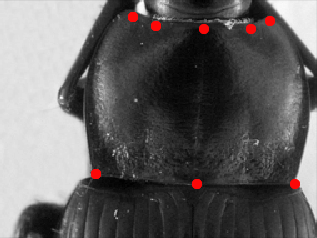
\includegraphics[width=0.35\textwidth]{images/fn_accuracy}}~~
\subfloat[Image with inaccuracy landmarks]{\label{figsub2}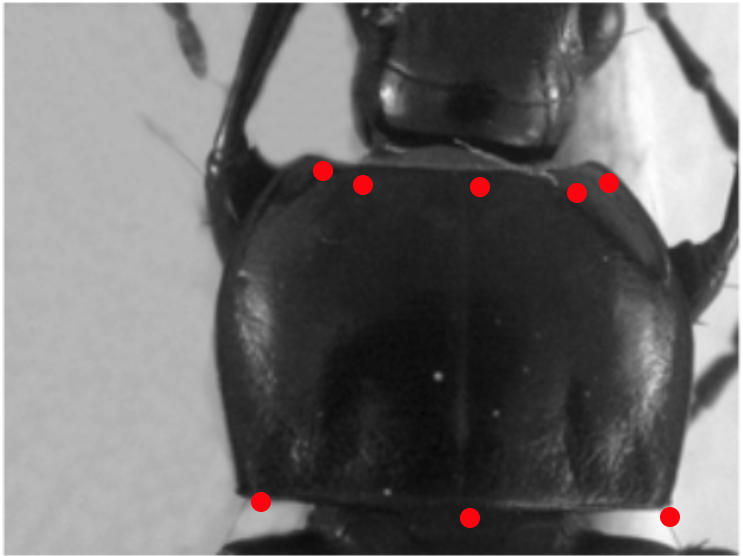
\includegraphics[width=0.35\textwidth]{images/plandmark2}}\\    
    \caption{The predicted landmarks, in red,  on the images in test set.}
    \label{figrsexample}
\end{figure}
\section{Improving results by fine-tuning}
\label{sfineTuning}
The results that we have been just discussed, have been obtained by
training EB-Net from scratch but training a network from scratch is
not the only way to work in Deep learning. It is possible to
initialize parameter values by extracting values from another
experiments with another dataset. This technique is called transfer learning
\cite{torrey2009transfer}. In transfer learning, the obtained
parameters values of a model, which have been used to solve a problem,
are reused for other datasets \cite{margeta_mri} and potentially to
solve another task. The name of this procedure is currently called
\textbf{fine-tuning}. 

Fine-tuning does not only replace and retrain the last layer of the model on
the new dataset but also tunes the weights of a trained model by
continuing the backpropagation. In this context, ImageNet
\cite{imagenet_cvpr09}, a well-known dataset with more than $100,000 $
images, has been used to train many famous CNN architectures such as
AlexNet \cite{krizhevsky2012imagenet} or VGG-16
\cite{simonyan2014very} with success. The pre-trained models on
ImageNet have been then shared in deep learning community as a source
to re-use features of ImageNet. Unfortunately, some preliminary tests
have shown that re-using ImageNet features is not relevant for our
application because as it has been described in by Lin et
al. \cite{lin2016homemade}, ImageNet features mainly concern the
detection of global shape of the objects whereas landmarks can be
considered as local features. Fortunately, searching for landmarks is
well defined in face recognition and facial key points detection, and 
we can consider that this application presents similarities with our problem. So,
we have decided to train EB-Net with a facial key points dataset and
then to transfer the trained parameters to fine-tune on beetle's
images.

\subsection{Pre-train EB-Net on Facial Keypoints dataset}
A \textbf{Facial Keypoints dataset} has been published for a
contest in the  Kaggle
community \footnote{https://www.kaggle.com/c/facial-key
  points-detection}. It includes $2,140$ human face images with the
size of $96 \times 96$. Each image contains $15$ landmarks on the
face: $6$ landmarks for eyes, $4$ landmarks for eyebrows, $4$
landmarks for mouth, and $1$ landmark for nose
tip. Fig. \ref{figaface} shows four face images in the dataset and the
landmarks on each face.

\begin{figure}[htbp]
	\centerline{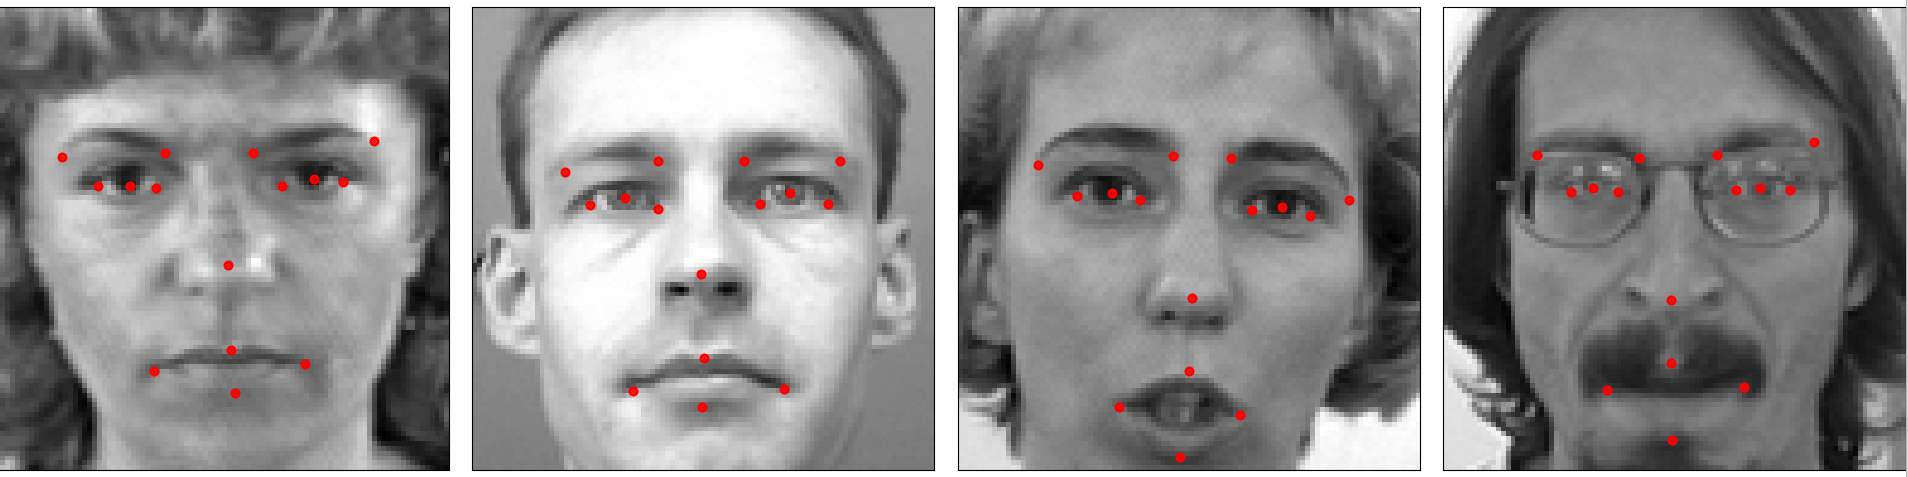
\includegraphics[scale=0.16]{images/face_dataset_2.png}}
	\caption{Four face images in the dataset and ground truth position of the landmarks.}
	\label{figaface}
\end{figure}

In our final experiment, EB-Net has been pre-trained with this dataset. The first objective of this task was to evaluate and to compare the
effectiveness of EB-Net with other published results in the
Kaggle challenge. Basically, the layer's parameters are the same than for
tranining from scratch, we have just adapted the image size in EB-Net
to match to $96 \times 96$ (Kaggle images size) and the output number of the last FC layer to
correspond to the waited number of landmarks ($15$
landmarks). Considering the EB-Net hyper-parameters, the learning rate and momentum remained the
same but the number of epochs has been increased to $10,000$ to improve the parameters learning. After training, the
obtained RMSE score is $1.1464$. This score is better than top $3$ on the leader board of this competition.

\subsection{Fine-tuning on beetle parts}
The fine-tuning stage was processed by transfering the layer parameters of
the pre-training step and by continuing the backpropagation. One can note that, the images in Facial Keypoints
dataset are squared, in order to respect this we have reduced the size
of beetle's images to $192 \times 192$ by cropping a background
band. To declare the difference between the Kaggle's images and the
beetle's ones, the stride property of the first convolutional
layer has been modified from $1$ to $2$.

After finishing the fine-tuning process, EB-Net was used to predict the
landmarks on test images. To evaluate the accuracy of the model's
outputs, the distances (in pixels) between predicted and corresponding
manual landmarks have been calculated again as their average
distances. Tables \ref{cmppronotum} resumes the results on pronotum
images: The ``\texttt{From scratch}" column reminds the previously average
distances when EB-Net was trained from scratch; the ``\texttt{Fine-tune}"
column presents the new average distances after applying
fine-tuning. The green and red values are respectively the best and
the worst average distances for each case. The same procedure has
been applied to the two others parts: elytra and head, the obtained results can be
seen in \ref{appdixA1}. First of all, the whole results have been clearly
improved with the help of transfer learning for each landmark. But to
go deeply in the analysis, it is worth to note that average computing can hide different situations, to have a look at that the distribution of the distances has been studied.

\begin{table}[htbp]
	\centering
	\begin{tabular}{|c|c|c|}
		\hline
		\textbf{$\#$LM} & \textbf{From scratch} & \textbf{Fine-tune} \\ \hline
		1 & \textcolor{green}{\textbf{4.00 }}& 2.99\\ \hline
		2 & 4.48 & 3.41  \\ \hline
		3 & 4.30  & 2.98 \\ \hline
		4 & 4.39  & 3.54\\ \hline
		5 & 4.29  & 3.37 \\ \hline
		6 & \textcolor{red}{\textbf{5.36}}  & \textcolor{red}{\textbf{4.06}} \\ \hline
		7 & 4.64  & \textcolor{green}{\textbf{2.93}} \\ \hline
		8 & 4.94  & 3.64 \\ \hline
	\end{tabular}
	\caption{Average distances comparison between training from scratch and fine-tuning on pronotum images}
	\label{cmppronotum}
\end{table}

Fig. \ref{figchartfn} describes the distribution of distances
of two examples cases: $1^{st}$ and $6^{th}$ landmarks, the best and the worst cases. Clearly, we can observe that the average distances have decreased by helping of fine-tuning in both the best and the worst cases, and the distribution of the distance points in the graphic is closest to the average value.

\begin{figure}[htbp]
    \centering
    \subfloat[$1^{st}$ landmark (from scratch)]{\label{}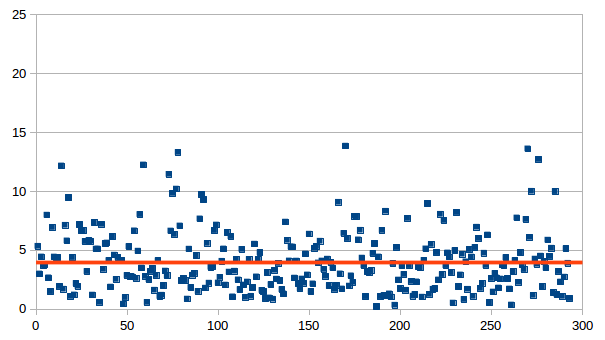
\includegraphics[width=0.49\textwidth]{images/charts/fs_lm1.png}}~~
    \subfloat[$6^{th}$ landmark (from scratch)]{\label{}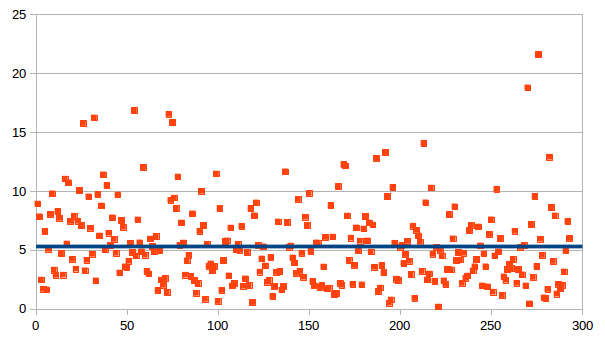
\includegraphics[width=0.49\textwidth]{images/charts/fs_lm6.png}}\\
    \subfloat[$1^{st}$ landmark (fine-tuning)]{\label{}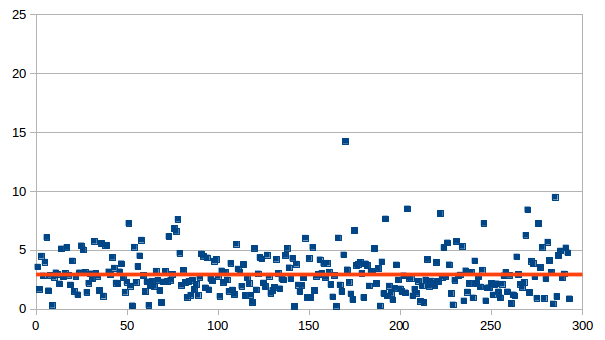
\includegraphics[width=0.49\textwidth]{images/charts/fn_lm1.png}}~~
    \subfloat[$6^{th}$ landmark (fine-tuning)]{\label{}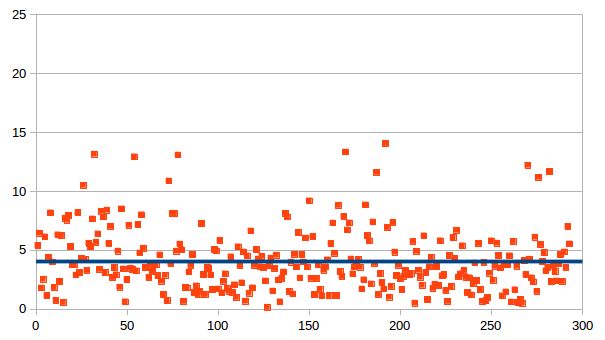
\includegraphics[width=0.49\textwidth]{images/charts/fn_lm6.png}}
    \caption{A comparison of distances distribution of the $1^{st}$ landmark and the $6^{th}$ landmark when applying two processes. The line in each figure presents the average distance value for these landmarks.}
    \label{figchartfn}
\end{figure}

As average distance reflects different situations, it is always interested to check also other statistical indicators to characterize the distribution of the distance values, such as standard error, median, minimum and maximum values. These
statistical values are presented in \ref{appdixA}. From these tables,
we can see the minimum and the maximum distances have a large range of
values. However, the median values, which separate the distances set
into two parts, are smaller than the averages values and they are very
close to the minimum values and so far from maximum values. It
confirms that almost all distances stay around the median values and
the predicted landmarks are good enough to replace the manual
ones. The distribution of the distances on each landmark of
each part are given in \ref{appdixB}. To illustrate the correctness of the approach, the Fig. \ref{figpdl} shows both the predicted (in red) and the manual (in yellow) landmarks for the three beetle parts.

\begin{figure}[h!]
    \centering
    \subfloat[Pronotum]{\label{}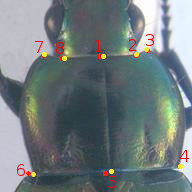
\includegraphics[width=0.45\textwidth]{images/predicted/Prono_001.JPG}}~~
    \subfloat[Head]{\label{}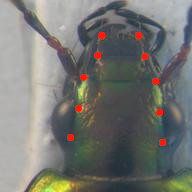
\includegraphics[width=0.45\textwidth]{images/predicted/Tete_005.JPG}}\\
	\subfloat[Elytra]{\label{}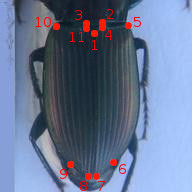
\includegraphics[width=0.45\textwidth]{images/predicted/Elytre004.JPG}}
    \caption{The location of predicted landmarks in one case of each part. The red/yellow points represent the predicted/manual landmarks.}
    \label{figpdl}
\end{figure}

The fine-tuning process has improved the results of the proposed
architecture on both $3$ sets of images: pronotum,
elytra and head. All the average distances have significantly
decreased: $\approx25.98\%$ on pronotum, $\approx15.8\%$ on elytra,
and $\approx18.10\%$  on head part. To evaluate the percentage of acceptable estimated landmarks, we validate all points with a distance from manual one less than the average plus standard error. With this procedure $\textbf{87.07\%}$ on pronotum,
$\textbf{87.92\%}$ on head, and $\textbf{91.78\%}$ on elytra, have been validated

\pagebreak
\section{Conclusion}
\label{sconclusion}
In this work, we have presented a new CNN model, EB-Net, to predict
key points, landmarks, on 2D anatomical images of beetles. EB-Net
model includes the repetition of $3$ Elementary Blocks, followed by
$3$ fully connected layers. Each elementary block is a sequence of $1$
CONV layer, $1$ maximum POOL layer and $1$ Dropout layer. In order to
augment the dataset size, we have generated new images by modification
of color channels of the original images. In the first strategy of the training step, EB-Net has been used to train and to test on the images of each part of beetle. While in the second strategy, transfer learning has been applied to improve the results. EB-Net has been trained on a human facial key points dataset before transfering to fine tune and to test on beetle's images.

To evaluate the predicted landmarks, the distances between them and corresponding manual ones have been computed. Then, the statistical indicators have been considered, such as: average distance, median distance, standard error, minimum and maximum distance. These values have figured out that using the convolutional network to predict the landmarks on biological images leads to satifying results without human intervention and procedures to pre-process (or post-process) the digital images. 

In both case of training from scratch and fine-tuning, most of predicted landmarks are close to the manual landmarks. The best set of estimated landmarks has been obtained after a step of fine-tuning using the whole set of images that we have for the
project, e.g. about all beetle parts. The quality of predicted coordinates allows using automatic landmarking to replace the manual ones.

\section*{References}

\bibliography{includes/mybibfile}

\pagebreak
\appendix
\section{Comparing the results between training from scratch and fine-tuning process}
\label{appdixA1}
Table \ref{cmptete} and \ref{cmpelytre} show the comparison of the average distance between two processes: training from scratch and fine-tuning, on each landmark of head and elytra images, respectively. The green and red numbers represent the best and the worst distances in each case.
\begin{table}[h]
	\begin{minipage}[t]{0.45\textwidth}
		\centering
		\begin{tabular}{|c|c|c|}
		\hline
		\textbf{$\#$LM} & \textbf{From scratch} & \textbf{Fine-tune} \\ \hline
		1 & \textcolor{red}{\textbf{5.53}} & \textcolor{red}{\textbf{4.82}}\\ \hline
		2 & 5.16 & 4.21 \\ \hline
		3 & 5.38  & 4.73 \\ \hline
		4 & 5.03  & 4.11 \\ \hline
		5 & \textcolor{green}{\textbf{4.18}}  & \textcolor{green}{\textbf{2.76}}\\ \hline
		6 & 4.45  & 3.50 \\ \hline
		7 & 4.79  & 3.92 \\ \hline
		8 & 4.53  & 3.40\\ \hline
		9 & 5.14  & 4.17 \\ \hline
		10 & 5.06  & 3.94\\ \hline
	\end{tabular}
	\caption{The average distance of two processes: training from scratch and fine-tuning, on each landmark of head images}
	\label{cmptete}
	\end{minipage}
	\hfill
	\begin{minipage}[t]{0.45\textwidth}
		\centering
		\begin{tabular}{|c|c|c|}
			\hline
			\textbf{$\#$LM} & \textbf{From scratch} & \textbf{Fine-tune} \\ \hline
			1 & \textcolor{green}{\textbf{3.87}} & 3.21  \\ \hline
			2 & 3.97 & 3.28 \\ \hline
			3 & 3.92  & \textcolor{green}{\textbf{3.20}}\\ \hline
			4 & \textcolor{green}{\textbf{3.87}}  & 3.22 \\ \hline
			5 & 4.02  & 3.31 \\ \hline
			6 & 4.84  & 4.21\\ \hline
			7 & 5.21  & 4.54 \\ \hline
			8 & \textcolor{red}{\textbf{5.47}}  & \textcolor{red}{\textbf{4.76}}\\ \hline
			9 & 5.27  & 4.55 \\ \hline
			10 & 4.07  & 3.39 \\ \hline
			11 & 3.99  & 3.29 \\ \hline
		\end{tabular}
		\caption{The average distance of two processes: training from scratch and fine-tuning, on each landmark of elytra images}
		\label{cmpelytre}
	\end{minipage}
\end{table}

\section{Statistic information on each beetle's part}
\label{appdixA}
Table \ref{a1}, \ref{a2}, and \ref{a3} display the statistical values on each part. The green and red numbers represent the best and the worst values on each statistical indicator, respectively.  
\begin{table}[htbp]
\begin{tabular}{ | c | c | c | c | c | c | }
\hline
	\textbf{\#LM} & \textbf{Mean} & \textbf{Standard Error} & \textbf{Median} & \textbf{Minimum} & \textbf{Maximum} \\ \hline
	LM1 & 2.9914 & \textcolor{green}{\textbf{0.1057}} & 2.7031 & \textcolor{red}{\textbf{0.23}} & 14.2496 \\ \hline
	LM2 & 3.4066 & 0.1306 & 2.9626 & 0.175 & 18.4053 \\ \hline
	LM3 & 2.9829 & 0.1205 & 2.5864 & 0.216 & 19.2092 \\ \hline
	LM4 & 3.5449 & 0.1422 & 3.117 & 0.1638 & \textcolor{red}{\textbf{22.8899}} \\ \hline
	LM5 & 3.3675 & 0.1327 & 2.9741 & \textcolor{green}{\textbf{0.101}} & 17.4586 \\ \hline
	LM6 & \textcolor{red}{\textbf{4.0611}} & \textcolor{red}{\textbf{0.1512}} & \textcolor{red}{\textbf{3.5733}} & 0.1733 & \textcolor{green}{\textbf{14.0745}} \\ \hline
	LM7 & \textcolor{green}{\textbf{2.9274}} & 0.1159 & \textcolor{green}{\textbf{2.5703}} & 0.2263 & 14.092 \\ \hline
	LM8 & 3.6448 & 0.145 & 3.0116 & 0.1647 & 15.4585 \\ \hline
\end{tabular}
\caption{The statistical indicator values on pronotum images}
\label{a1}
\end{table}

\begin{table}[htbp]
\begin{tabular}{ | c | c | c | c | c | c | }
\hline
	\textbf{\#LM} & \textbf{Mean} & \textbf{Standard Error} & \textbf{Median} & \textbf{Minimum} & \textbf{Maximum} \\ \hline
	LM1 & \textcolor{red}{\textbf{4.8185}} & 0.1709 & 4.2951 & 0.3732 & 21.1819 \\ \hline
	LM2 & 4.2098 & \textcolor{red}{\textbf{0.1715}} & 3.7484 & 0.2072 & \textcolor{red}{\textbf{23.9351}} \\ \hline
	LM3 & 4.7286 & 0.1705 & \textcolor{red}{\textbf{4.3991}} & 0.2719 & \textcolor{green}{\textbf{19.12}} \\ \hline
	LM4 & 4.1071 & 0.1701 & 3.6232 & 0.1942 & 21.6451 \\ \hline
	LM5 & 4.1769 & 0.1545 & 3.7967 & 0.2683 & 20.2307 \\ \hline
	LM6 & 3.4976 & 0.1657 & 2.9338 & 0.2384 & 22.6836 \\ \hline
	LM7 & 3.9168 & \textcolor{green}{\textbf{0.1477}} & 3.4284 & 0.2134 & 21.0319 \\ \hline
	LM8 & \textcolor{green}{\textbf{3.402}} & 0.1486 & \textcolor{green}{\textbf{2.7877}} & \textcolor{green}{\textbf{0.1478}} & 21.233 \\ \hline
	LM9 & 4.1703 & 0.1481 & 3.7181 & \textcolor{red}{\textbf{0.4441}} & 22.0267 \\ \hline
	LM10 & 3.9433 & 0.1574 & 3.4147 & 0.152 & 20.7223 \\ \hline
\end{tabular}
\caption{The statistical indicator values on head images}
\label{a2}
\end{table}

\begin{table}[htbp]
	\begin{tabular}{ | c | c | c | c | c | c | }
\hline
	 \textbf{\#LM} & \textbf{Mean} & \textbf{Standard Error} & \textbf{Median} & \textbf{Minimum} & \textbf{Maximum} \\ \hline
	LM1 & 3.2081 & 0.179 & 2.6311 & 0.1265 & 32.6688 \\ \hline
	LM2 & 3.2842 & 0.1872 & 2.5934 & 0.1607 & 33.9982 \\ \hline
	LM3 & \textcolor{green}{\textbf{3.1975}} & \textcolor{green}{\textbf{0.1755}} & 2.5412 & 0.0763 & 31.0928 \\ \hline
	LM4 & 3.225 & 0.1812 & \textcolor{green}{\textbf{2.479}} & 0.1485 & 33.1458 \\ \hline
	LM5 & 3.3062 & 0.1869 & 2.606 & 0.1187 & \textcolor{red}{\textbf{35.7959}} \\ \hline
	LM6 & 4.2069 & 0.1957 & 3.578 & 0.2149 & 35.3037 \\ \hline
	LM7 & 4.5445 & \textcolor{red}{\textbf{0.2049}} & 4.0792 & 0.3454 & 34.7368 \\ \hline
	LM8 & \textcolor{red}{\textbf{4.7596}} & 0.2018 & \textcolor{red}{\textbf{4.3057}} & \textcolor{red}{\textbf{0.4697}} & 32.1749 \\ \hline
	LM9 & 4.548 & 0.1916 & 3.9626 & 0.2711 & \textcolor{green}{\textbf{28.3484}} \\ \hline
	LM10 & 3.3918 & 0.1772 & 2.7726 & 0.1799 & 29.9211 \\ \hline
	LM11 & 3.2897 & 0.1764 & 2.7064 & \textcolor{green}{\textbf{0.0527}} & 32.3641 \\ \hline
\end{tabular}
\caption{The statistical indicator values on elytra images}
\label{a3}
\end{table}

\pagebreak
\section{The distribution of distances on each part}
\label{appdixB}
The Figure \ref{dtpronotum}, \ref{dthead}, and \ref{dtelytre} illustrate the distribution of distances on each landmark of each part: pronotum, head, and elytra, respectively. The red line represents the mean value of the distance in each case.
\begin{figure}[htbp]
    \centering
    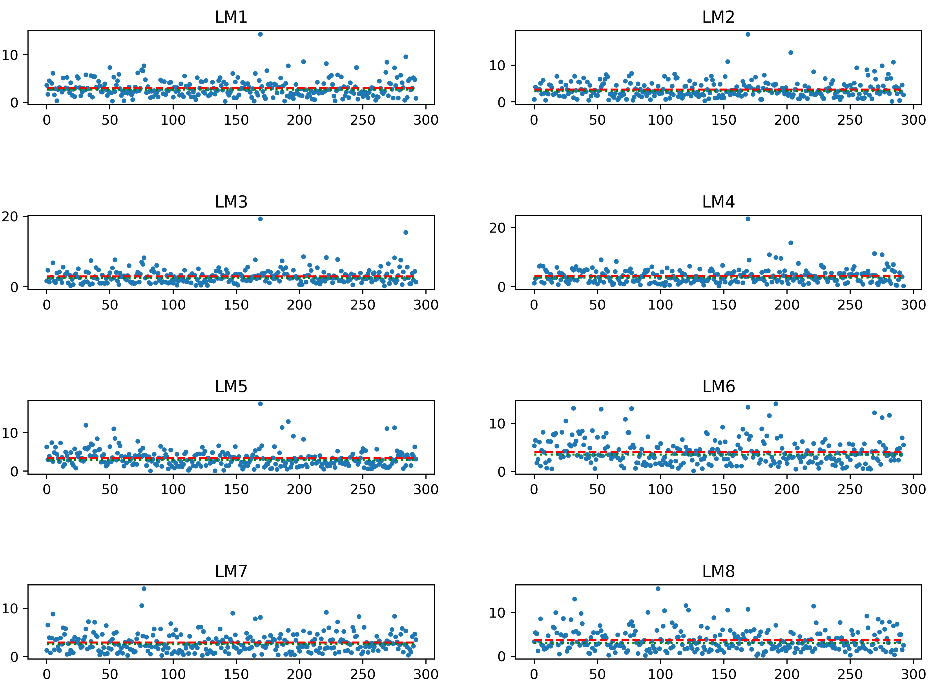
\includegraphics[width=.95\textwidth]{images/charts/pronotum_2.png}
    \caption{The distribution of distances on each landmark of all pronotum images}
    \label{dtpronotum}
\end{figure}

\begin{figure}[htbp]
    \centering
    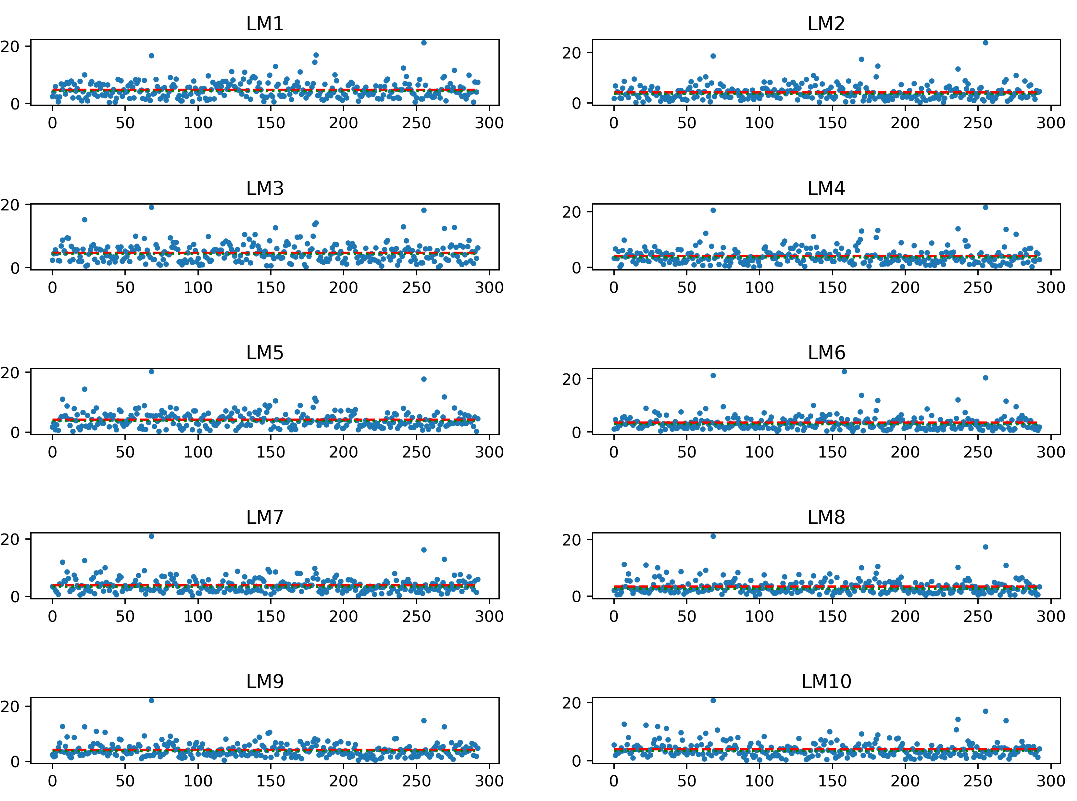
\includegraphics[width=.95\textwidth]{images/charts/tete_2.png}
    \caption{The distribution of distances on each landmark of all head images}
    \label{dthead}
\end{figure}

\begin{figure}[htbp]
    \centering
    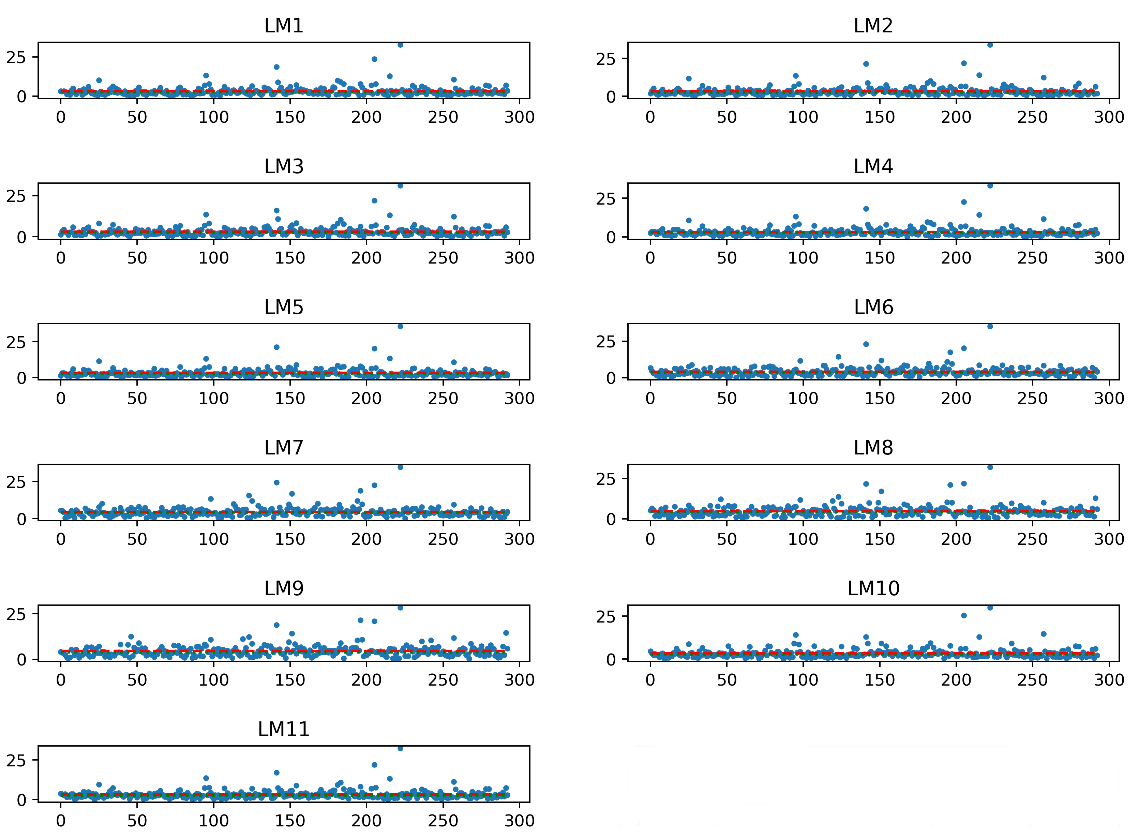
\includegraphics[width=.95\textwidth]{images/charts/elytre_2.png}
    \caption{The distribution of distances on each landmark of all elytra images}
    \label{dtelytre}
\end{figure}
\end{document}

We have also a comparison between the results of deep learning and
early methods where we have applied image processing techniques to
predict the landmarks \cite{le2017maelab}. Clearly, the result with
fine-tuning has improved the location of estimated landmarks. Even the
average distances obtained from scratch training are still higher but
they are more stable than the results from the early method: most of
the average distance(or landmarks) of left mandibles are less than the
results of the early method, while the average distances are very
close in the case of right mandibles.

Additionally, if we consider a
predicted landmark, which has the distance (from manual ones) less
than mean value plus standard deviation, is acceptable, the accuracy
of method on each part is $\textbf{87.07\%}$ on pronotum,
$\textbf{87.92\%}$ on head, and $\textbf{91.78\%}$ on elytra.
